\newcommand{\svcourse}{CST Part IA: Software Engineering and Security}
\newcommand{\svnumber}{1}
\newcommand{\svvenue}{Microsoft Teams}
\newcommand{\svdate}{2022-05-11}
\newcommand{\svtime}{15:00}
\newcommand{\svuploadkey}{CBd13xmL7PC1zqhNIoLdTiYUBnxZhzRAtJxv/ytRdM1r7qIfwMsxeVwM/pPcIo8l}

\newcommand{\svrname}{Dr Sam Ainsworth}
\newcommand{\jkfside}{oneside}
\newcommand{\jkfhanded}{yes}

\newcommand{\studentname}{Harry Langford}
\newcommand{\studentemail}{hjel2@cam.ac.uk}


\documentclass[10pt,\jkfside,a4paper]{article}

% DO NOT add \usepackage commands here.  Place any custom commands
% into your SV work files.  Anything in the template directory is
% likely to be overwritten!

\usepackage{fancyhdr}

\usepackage{lastpage}       % ``n of m'' page numbering
\usepackage{lscape}         % Makes landscape easier

\usepackage{verbatim}       % Verbatim blocks
\usepackage{listings}       % Source code listings
\usepackage{graphicx}
\usepackage{float}
\usepackage{epsfig}         % Embed encapsulated postscript
\usepackage{array}          % Array environment
\usepackage{qrcode}         % QR codes
\usepackage{enumitem}       % Required by Tom Johnson's exam question header

\usepackage{hhline}         % Horizontal lines in tables
\usepackage{siunitx}        % Correct spacing of units
\usepackage{amsmath}        % American Mathematical Society
\usepackage{amssymb}        % Maths symbols
\usepackage{amsthm}         % Theorems

\usepackage{ifthen}         % Conditional processing in tex

\usepackage[top=3cm,
            bottom=3cm,
            inner=2cm,
            outer=5cm]{geometry}

% PDF metadata + URL formatting
\usepackage[
            pdfauthor={\studentname},
            pdftitle={\svcourse, SV \svnumber},
            pdfsubject={},
            pdfkeywords={9d2547b00aba40b58fa0378774f72ee6},
            pdfproducer={},
            pdfcreator={},
            hidelinks]{hyperref}

\renewcommand{\headrulewidth}{0.4pt}
\renewcommand{\footrulewidth}{0.4pt}
\fancyheadoffset[LO,LE,RO,RE]{0pt}
\fancyfootoffset[LO,LE,RO,RE]{0pt}
\pagestyle{fancy}
\fancyhead{}
\fancyhead[LO,RE]{{\bfseries \studentname}\\\studentemail}
\fancyhead[RO,LE]{{\bfseries \svcourse, SV~\svnumber}\\\svdate\ \svtime, \svvenue}
\fancyfoot{}
\fancyfoot[LO,RE]{For: \svrname}
\fancyfoot[RO,LE]{\today\hspace{1cm}\thepage\ / \pageref{LastPage}}
\fancyfoot[C]{\qrcode[height=0.8cm]{\svuploadkey}}
\setlength{\headheight}{22.55pt}


\ifthenelse{\equal{\jkfside}{oneside}}{

 \ifthenelse{\equal{\jkfhanded}{left}}{
  % 1. Left-handed marker, one-sided printing or e-marking, use oneside and...
  \evensidemargin=\oddsidemargin
  \oddsidemargin=73pt
  \setlength{\marginparwidth}{111pt}
  \setlength{\marginparsep}{-\marginparsep}
  \addtolength{\marginparsep}{-\textwidth}
  \addtolength{\marginparsep}{-\marginparwidth}
 }{
  % 2. Right-handed marker, one-sided printing or e-marking, use oneside.
  \setlength{\marginparwidth}{111pt}
 }

}{
 % 3. Alternating margins, two-sided printing, use twoside.
}


\setlength{\parindent}{0em}
\addtolength{\parskip}{1ex}

% Exam question headings, labels and sensible layout (courtesy of Tom Johnson)
\setlist{parsep=\parskip, listparindent=\parindent}
\newcommand{\examhead}[3]{\section{#1 Paper #2 Question #3}}
\newenvironment{examquestion}[3]{
\examhead{#1}{#2}{#3}\setlist[enumerate, 1]{label=(\alph*)}\setlist[enumerate, 2]{label=(\roman*)}
\marginpar{\href{https://www.cl.cam.ac.uk/teaching/exams/pastpapers/y#1p#2q#3.pdf}{\qrcode{https://www.cl.cam.ac.uk/teaching/exams/pastpapers/y#1p#2q#3.pdf}}}
\marginpar{\footnotesize \href{https://www.cl.cam.ac.uk/teaching/exams/pastpapers/y#1p#2q#3.pdf}{https://www.cl.cam.ac.uk/\\teaching/exams/pastpapers/\\y#1p#2q#3.pdf}}
}{}


\usepackage{caption}
\usepackage{subcaption}
\usepackage{graphicx}
\usepackage{float}
\usepackage{tikz}
\usepackage{pythonhighlight}
\usepackage{wasysym}
\usetikzlibrary{automata, positioning, arrows}

\newcommand{\idastar}{\text{IDA}\ensuremath{^*}}

\tikzset{
->,
>=stealth,
node distance=3cm,
every state/.style={thick, fill=gray!10},
initial text=$ $,
}

\newcommand{\astar}{\ensuremath{A^\star}}

\begin{document}

\part{Sean's Exercise Sheet Part 1}

\setcounter{section}{2}

\section{Search}

\begin{enumerate}

\item Explain why breadth-first search is optimal if path-cost is a
non-decreasing function of node depth.

Breadth-first search searches in order of depth; if the first
goal node found by breadth-first search $n_g$ is found at depth $d_g$ then
any goal nodes $n_g'$ found later will be found at depth $d_g' \ge d_g$.

Since path-cost is a non-decreasing function of node depth, we have for some
non-decreasing function $f$, $p(n_g) = f(d_g) \le f(d_g') = p(n_g')$. So
$p(s_g) \le p(s_g')$. Therefore, the first goal node will have a lower path
cost than any goal nodes found later. Hence breadth-first search is optimal
under the assumption that path-cost is a non-decreasing function of node
depth.

\item In the graph search algorithm, assume a node is taken from the fringe
and found \textit{not} to be a goal and \textit{not} to be in
\texttt{closed}. We then add it to \texttt{closed} and add its descendants
to \texttt{fringe}.

\begin{enumerate}[label=(\alph*)]

\item When might it make sense to add \textit{all} descendants to the queue
without checking if they are in \texttt{closed} first?

It would make sense to add all descendants to the queue without checking if
they are in \texttt{closed} if we knew the graph we were searching was a
tree. In a tree there is only one path from the root to any node. So we
would know that none of the descendants would be in \texttt{closed} --
making it a redundant test.

% TODO "we need this check to make sure its optimal"

\item Explain why the code in the lecture notes has been changed to add
descendants to the queue only if they are not already in \texttt{closed}.

The code in the lecture notes is a \textit{graph} search algorithm -- it
aims to work on all graphs. So should not have problem-specific
optimisations.

If this check was not present, searches on undirected (or cyclic) graphcs
would no longer be complete. For example a DFS on an undirected graph would
loop infinitely on the first two nodes.

\end{enumerate}

\item Iterative deepening depends on the fact that \textit{the vast majority of
the nodes in a tree are in the bottom level}.

\begin{itemize}

\item Denote by $f_1(b, d)$ the total number of nodes appearing in a tree
with branching factor $b$ and depth $d$. Find a closed-form expression for
$f_1(b, d)$.

\[
\begin{split}
f_1(b, d)
&= \sum^d_{i=0} b^i \\
&= \frac{b^{d + 1} - 1}{b - 1}
\end{split}
\]

\item Denote by $f_2(b, d)$ the total number of nodes generated in a
complete iterative deepening search to depth $d$ of a tree having branching
factor $b$. Find a closed-form expression for $f_2(b, d)$ in terms of
$f_1(b, d)$.

\[
\begin{split}
f_2(b, d)
&= \sum^{d}_{i=0} f_1(b, i) \\
&= \sum^{d}_{i=0} \frac{b^{i + 1} - 1}{b - 1} \\
&= \frac{1}{b - 1} \left( \sum^{d}_{i=0} b^{i+1} - 1 \right) \\
&= \frac{1}{b - 1} \left(\left(b\sum^{d}_{i=0} b^{i+1}\right) - d - 1\right) \\
&= \frac{1}{b-1}\left( b\frac{b^{d + 1} - 1}{b - 1} - d - 1\right) \\
&= \frac{b^{d + 2} - b - bd + d - b + 1}{(b - 1)^2}
\end{split}
\]

\item How do $f_1(b, d)$ and $f_2(b, d)$ compare when $b$ is large?

For large $b$, $f_1(b, d) \approx f_2(b, d)$.

\end{itemize}

\item The \astar algorithm does not perform a goal test on any state 
\textit{until it has selected it for expansion}. We might consider a 
slightly different approach: namely, each time a node is expanded check all 
of its descendants to see if they include a goal.

Give two reasons why this is a misguided idea, where possible illustrating 
your answer using a specific example of a search tree for which it would be 
problematic.

\begin{itemize}

\item Under the alternative algorithm, we no longer test nodes in ascending
order of estimated cost. This means, \textit{even with monotonic heuristics}
the algorithm will not be optimal. The first node we test may be a highly
suboptimal goal state or have been found by a highly suboptimal path.

Consider the graph below:
\begin{figure}[H]
\centering
\begin{tikzpicture}
\node [state] (s0)
{$\begin{matrix} s_0 \\ h = 2 \end{matrix}$};
\node [state, below left = 2 of s0] (s1)
{$\begin{matrix} s_1 \\ h = 1 \end{matrix}$};
\node [state, below right = 2 of s0] (s2)
{$\begin{matrix} s_2 \\ h = 1 \end{matrix}$};
\node [state, accepting, below = 2 of s1] (s3)
{$\begin{matrix} s_3 \\ h = 0 \end{matrix}$};
\node [state, accepting, below = 2 of s2] (s4)
{$\begin{matrix} s_4 \\ h = 0 \end{matrix}$};
\node [left = 0.5 of s0] (start) {};
\path (start) edge (s0);
\path
(s0) edge [above left] node (c01) {$2$} (s1)
(s0) edge [above right] node (c02) {$1$} (s2)
(s1) edge [left] node (c13) {$1$} (s3)
(s2) edge [right] node (c24) {$10$} (s4);
\end{tikzpicture}
\caption{Graph on which alternative A$^*$ finds a non-optimal goal}
\end{figure}

In this example, the heuristic is both admissible and monotonic. However,
since it underestimates the cost of $s_2$ more than $s_1$, $s_2$ is explored
and expanded first, leading to a highly suboptimal goal.

\item Consider an example where testing for a goal state is computationally
expensive (i.e involves running a simulation) -- but we have a very good
monotonic heuristic. If the graph has a high branching factor, then the
cost of searching the graph becomes dominated by unnecessary tests for goal
states -- this ``optimisation'' increases compute-time by a factor of $b-1$.

\end{itemize}

\item The $f$-cost is defined in the usual way as
\[
f(n) = p(n) + h(n)
\]
where $n$ is any node, $p$ denotes path cost and $h$ denotes the heuristic. 
An admissible heuristic is one which, for any $n$
\[
h(n) \le \text{actual distance from $n$ to the goal}
\]
and a heuristic is monotonic if for consecutive nodes $n$ and $n'$ it is 
always the cast that
\[
f(n') \ge f(n)
\]
\begin{itemize}

\item Prove that $h$ is monotonic if and only if it obeys the triangle 
inequality, which states that for any consecutive nodes $n$ and $n'$
\[
h(n) \le c_{n \to n'} + h(n)
\]
where $c_{n \to n'}$ is the cost of moving from $n$ to $n'$.

Assume $h$ is monotonic:
\[
\begin{split}
f(n) &\le f(n') \\
p(n) + h(n) &\le p(n') + h(n') \\
p(n) + h(n) &\le p(n) + c_{n \to n'} + h(n') \\
h(n) &\le c_{n \to n'} + h(n')
\end{split}
\]
Therefore, if $h$ is monotonic, then it obeys the triangle inequality.

Assume $h$ obeys the triangle inequality:
\[
\begin{split}
h(n) &\le c_{n \to n'} + h(n') \\
p(n) + h(n) &\le p(n) + c_{n \to n'} + h(n') \\
p(n) + h(n) &\le p(n') + h(n') \\
f(n) &\le f(n') \\
\end{split}
\]
Therefore, if $h$ obeys the triangle inequality then it is monotonic.

Since we have proved both directions, we have that $h$ is monotonic if and
only if it obeys the triangle inequality.

\item Prove that if a heuristic is monotonic then it is also admissible

Assume a heuristic is monotonic.

Next, assume there is a path $n_0 \to n_1 \to \dots \to n_k$ for some
node $n_0$ and some goal node $n_k$. Using monotonicity, we have:
\[
\begin{split}
f(n_0) &\le f(n_1) \le \dots \le f(n_k) \\
f(n_0) &\le f(n_k) \\
p(n_0) + h(n_0) &\le p(n_0) + h'(n_0) \\
h(n_0) &\le h'(n_0)
\end{split}
\]
This is the admissibility property. Therefore, if a heuristic is monotonic
then it is also admissible.

\item Is the converse true? Either prove that this is the case or provide a 
counterexample.

The converse is not true. I provide an example where the heuristic is
admissible, but not monotonic.

\begin{figure}[H]
\centering
\begin{tikzpicture}
\node [state, minimum size = 1.5cm] (start)
{$\begin{matrix} s_0 \\ h = 5\end{matrix}$};
\node [state, minimum size = 1.5cm, right = of start] (mid)
{$\begin{matrix} x_1 \\ h = 3 \end{matrix}$};
\node [state, minimum size = 1.5cm, right = of mid, accepting] (goal)
{$\begin{matrix} goal \\ h = 0 \end{matrix} $};
\draw (start) edge [above] node {$c_{s_0 \to s_1} = 3$} (mid)
(mid) edge [above] node {$c_{s_1 \to goal} = 3$} (goal);
\end{tikzpicture}
\caption{Counterexample to Admissibility implying Monotonicity}
\end{figure}

\end{itemize}

\setcounter{enumi}{6}

\item In some problems we can simultaneously search:
\begin{itemize}

\item \textit{forward} form the \textit{start} state

\item \textit{backwards} from the \textit{goal} state

\end{itemize}
until the searches meet. This seems like it might be a very good idea:
\begin{itemize}

\item If the search methods have complexity $\mathcal O\left(b^d\right)$
then\ldots

\item \ldots we are converting this to $\mathcal O\left( 2 b^{d/2} \right) =
\mathcal O\left( b^{d/2} \right) $.

\end{itemize}
(Here, we are assuming the branching factor is $b$ in both directions). Why
might this not be as good an idea as it seems?

In the general case, the start state is not known in advance. This may
make a ``good'' heuristic for the distance \textit{to} the start state
impossible to automatically generate.

Furthermore, even if we were to make such a heuristic; there is no guarantee
that the forward and reverse seearches would meet at an optimal node.
In-fact it would be impossible (in the general case) to even prove a
\textit{bound} on how suboptimal the solution we found was.

Therefore, the algorithm would require human intervention (to make a good
heuristic) and would no longer give an optimal path cost -- or a
near-optimal path cost.

There are obviously edge-cases where one or both of these problems do not
apply.

\item Suggest a method for performing depth-first search using only
$\mathcal O(d)$ space.

The algorithm I provide is designed to search a graph in $\mathcal O(d)$
space. Searching a tree in $\mathcal O(d)$ space is trivial. This algorithm
works by considering the graph as a tree -- this means it may revisit nodes.

\begin{python}
def dfs(n: node, seen: set[node]):
	if goal(node):
		return node
	for neighbour in node.neighbours:
		if neighbour not in seen:
			dfs(neighbour, seen | {neighbour})
\end{python}

\item One modification to the basic local search algorithm suggested in the
lectures was to make steps probabilistically, but only if the value of $f$
is \textit{improved}.
\begin{enumerate}[label=(\alph*)]

\item Would it be a good idea to also allow steps that move to a state with
a \textit{worse} value for $f$?

Yes. In cases where the function state space $f$ is not well-behaved
(contains local maxima), we may be able to find a more optimal solution if
we explore parts of the graph appear to be slightly worse in the short-term.
However, under this strategy we may wish to remember the best state we have
found in-case this exploration does not yield a better state.

\item Suggest an algorithm for achieving this such that you have some
control between steps that increase or decrease $f$.

I propose an algorithm similar to simulated annealing:
\begin{lstlisting}[language=Python, mathescape=true]
def anneal($s_0$, f, $t_{\max}$, $\delta$):
    $s$ = $s_0$
    $t$ = $t_{\max}$
    best = $s_0$
    while True:
        best = max(best, max($s$.neighbours, key=f), key=f)
        $w$ = [$f(s')$ + $t$ - $f(s)$ for $s'$ in $s$.neighbours]
        $p$ = [$f_{s'}$ / sum($w$) for $s'$ in $w$ if $f_{s'}$ > 0]
        if not p:
        	return best
        $s$ = random.choice($s$.neighbours, $p$)
	$t$ -= $\delta$
\end{lstlisting}

% TODO simulated annealing with temperature?

\end{enumerate}

\end{enumerate}

\part{Sean's Exercise Sheet Part 2}

\setcounter{section}{0}

\section{Games}

\begin{enumerate}

\item Consider the following game tree:

\begin{figure}[H]
\centering
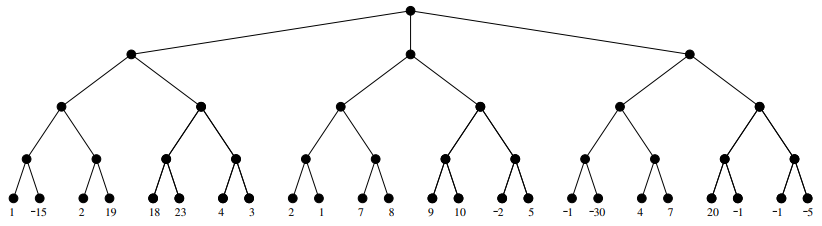
\includegraphics[width=0.6\textwidth]{minmaxtree}
\end{figure}

Large outcomes are beneficial for Max. How is the tree pruned by $\alpha -
\beta$ minimax if Max moves first? How is it pruned if Min is the root, and
therefore moves first.

Using $i, j$ as an abbreviation for $\alpha = i$, $\beta = j$:

\begin{figure}[H]
\centering
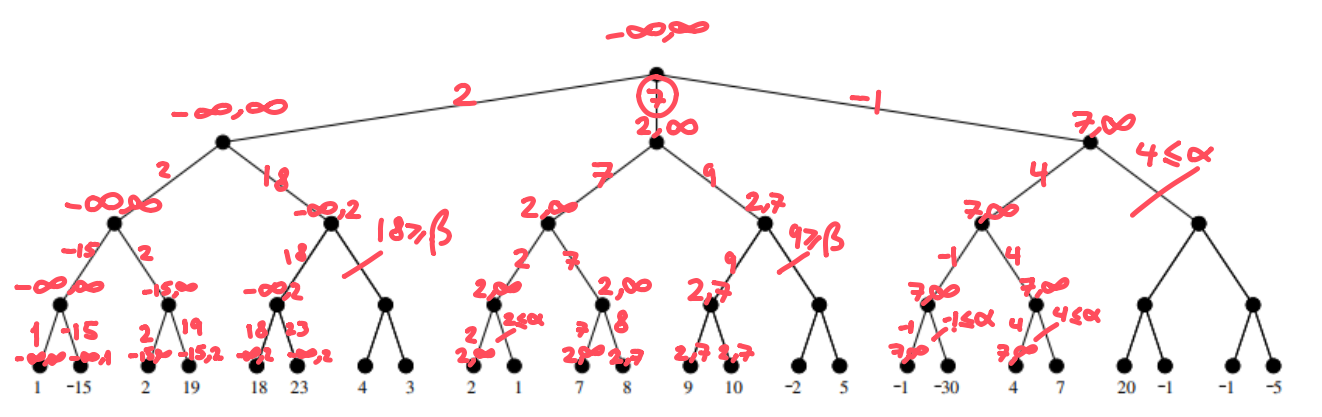
\includegraphics[width=\textwidth]{maxtree}
\caption{Max achieves 7}
\end{figure}

\begin{figure}[H]
\centering
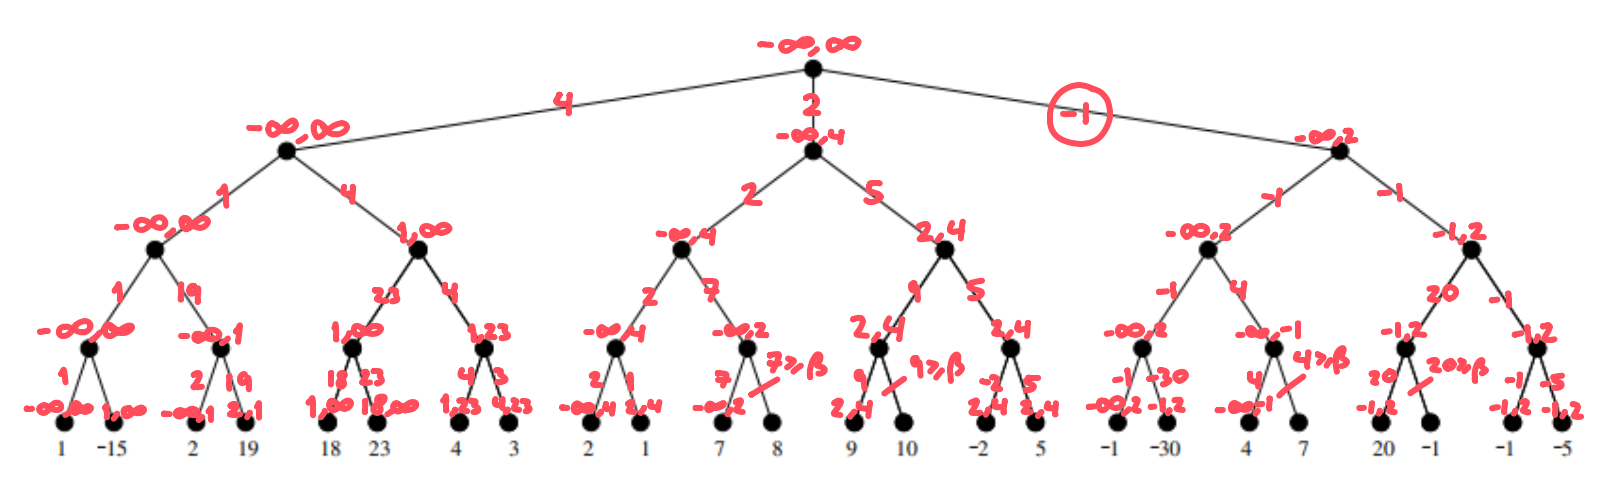
\includegraphics[width=\textwidth]{mintree}
\caption{Min achieves -1}
\end{figure}

\setcounter{enumi}{2}

\item Is the minimax approach to playing games optimal against an imperfect
opponent? Either prove this is the case or give a counterexample.

This depends on our definition of ``optimal''; and in what way the opponent
is imperfect. If the opponent has a nonzero probability of making any move
and our definition of ``optimal'' is ``the move which maximises the
worst-case outcome'', then minimax is optimal.

If our definition of ``optimal'' is ``maximising expected utility'' then
minimax may not be optimal.

Additionally, if our opponent has a zero probability of making some moves (i.e
because of an affection heuristic, they never move left on binary branches)
then minimax is not optimal. In the figure below, minimax would find a
solution with utility 0 for Max. If we exploit Min's affection heuristic,
Max could achieve a utility of 1.

\begin{figure}[H]
\centering
\begin{tikzpicture}
\draw [black, fill=black] (0, 0) circle (.5ex);
\draw [black, fill=black] (-1, -1) circle (.5ex);
\draw [black, fill=black] (1, -1) circle (.5ex);
\draw [black, fill=black] (-1.5, -2) circle (.5ex);
\draw [black, fill=black] (-0.5, -2) circle (.5ex);
\draw [black, fill=black] (0.5, -2) circle (.5ex);
\draw [black, fill=black] (1.5, -2) circle (.5ex);
\node (node0) at (-1.5, -2.5) {0};
\node (node0) at (-0.5, -2.5) {0};
\node (node0) at (0.5, -2.5) {-1};
\node (node0) at (1.5, -2.5) {1};
\path [-]
(0, 0) edge (-1, -1)
(0, 0) edge (1, -1)
(-1, -1) edge (-1.5, -2)
(-1, -1) edge (-0.5, -2)
(1, -1) edge (1.5, -2)
(1, -1) edge (0.5, -2);
\end{tikzpicture}
\end{figure}

\end{enumerate}

\section{Constraint Satisfaction Problems}

\begin{enumerate}

\item Consider the following constraint satisfaction problem:
\begin{figure}[H]
\centering
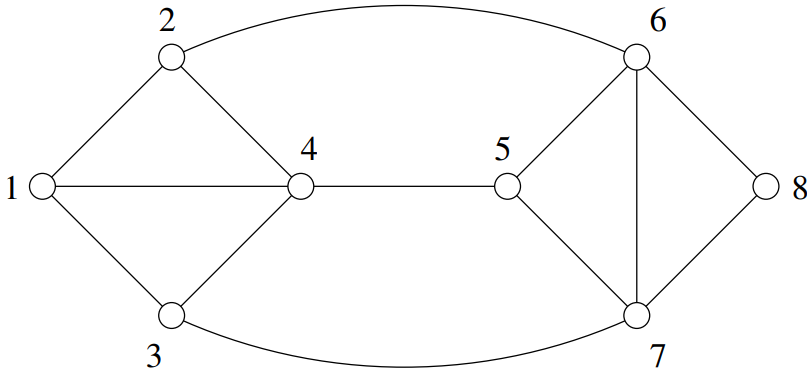
\includegraphics[width=0.6\textwidth]{constraintsat}
\end{figure}
We want to colour the nodes using the colours red (R), cyan (C) and black
(B) in such a way that connected nodes have different colours.
\begin{itemize}

\item Assuming we attempt the assignments $1 = R$, $4 = C$, $5 = R$, $8 =
C$, $6 = B$. Explain how \textit{forward checking} operates in this example,
and how it detects the need to backtrack.

In forward-checking, after assigning a node a value, we remove this value
from the domain of all adjacent nodes. An partial instantiation $I_k$ of $k$
variables is said to conflict with node $V_i$ if, under forward checking
$V_i$ has no valid assignments. Once any node conflicts with the current
partial initialisation, partial checking will determine that the search
cannot succeed and will backtrack.

Under forward checking (after making the first 4 assignments) the graph
would be in the following state:

\begin{table}[H]
\centering
\begin{tabular}{c|c|c}
node & assigned & values \\
\hline
1 & $R$ & $\{R\}$ \\
2 & & $\{B\}$ \\
3 & & $\{B\}$ \\
4 & $C$ & $\{C\}$ \\
5 & $R$ & $\{R\}$ \\
6 & & $\{B\}$ \\
7 & & $\{B\}$ \\
8 & $C$ & $\{C\}$
\end{tabular}
\end{table}

Once the search attempted to assign $6 = B$, it would remove $B$ from the
possible values of all adjacent nodes. This would leave the graph in the
following state:

\begin{figure}[H]
\centering
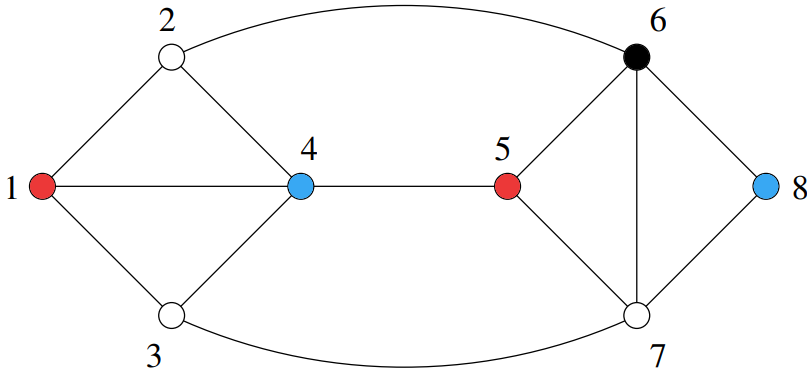
\includegraphics[width=0.6\textwidth]{constraintsat2}
\end{figure}

\begin{table}[H]
\centering
\begin{tabular}{c|c|c}
node & assigned & values \\
\hline
1 & $R$ & $\{R\}$ \\
2 & & $\{\}$ \\
3 & & $\{B\}$ \\
4 & $C$ & $\{C\}$ \\
5 & $R$ & $\{R\}$ \\
6 & $B$ & $\{B\}$ \\
7 & & $\{\}$ \\
8 & $C$ & $\{C\}$
\end{tabular}
\end{table}

On assigning $6 = B$, forward checking would check that this was consistent
with some value on all adjacent nodes. It would then backtrack to $8 = C$
and try $8 = B$, continuing the search.

\item Will the AC-3 algorithm detect a problem earlier in this case? Explain
the operation of the algorithm in the example.

The AC-3 algorithm would detect a problem earlier in this case. The AC-3
algorithm is a way of implementing constraint propogation. It ensures that
for all edges $V_i \to V_j$, $V_i$ is consistent with $V_j$. This means that
for all assignments of $V_i$, there exists an assignment to $V_j$ which is
consistent with that. If this is not the case, AC-3 will remove this value
from the set of possible values of $V_i$ -- and then recursively check all
edges $V_k \to V_i$ for consistency.

After assigning $1 = R$, the possible values are as follows:

\begin{table}[H]
\centering
\begin{tabular}{c|c|c}
node & assigned & values \\
\hline
1 & $R$ & $\{R\}$ \\
2 & & $\{B, C\}$ \\
3 & & $\{B, C\}$ \\
4 & & $\{B, C\}$ \\
5 & & $\{R, B, C\}$ \\
6 & & $\{R, B, C\}$ \\
7 & & $\{R, B, C\}$ \\
8 & & $\{R, B, C\}$ \\
\end{tabular}
\end{table}

After assigning $4 = C$, the possible values (under AC-3) are as follows:

\begin{table}[H]
\centering
\begin{tabular}{c|c|c}
node & assigned & values \\
\hline
1 & $R$ & $\{R\}$ \\
2 & & $\{B\}$ \\
3 & & $\{B\}$ \\
4 & $C$ & $\{C\}$ \\
5 & & $\{R, B, C\}$ \\
6 & & $\{R, C\}$ \\
7 & & $\{R, C\}$ \\
8 & & $\{R, B, C\}$ \\
\end{tabular}
\end{table}

After assigning $5 = R$, the possible values are as follows:

\begin{table}[H]
\centering
\begin{tabular}{c|c|c}
node & assigned & values \\
\hline
1 & $R$ & $\{R\}$ \\
2 & & $\{B\}$ \\
3 & & $\{B\}$ \\
4 & $C$ & $\{C\}$ \\
5 & $R$ & $\{R\}$ \\
6 & & $\{C\}$ \\
7 & & $\{C\}$ \\
8 & & $\{R, B\}$ \\
\end{tabular}
\end{table}

AC-3 has determined that $C$ is not a consistent value for $8$ to take. So
AC-3 notices that the current assignment is inconsistent earlier and
backtracks earlier.

\end{itemize}

\end{enumerate}

\part{Exam Questions}

\setcounter{section}{0}

\begin{examquestion}{2016}{4}{2}

\begin{enumerate}[label=(\alph*)]

\item Provide a detailed description of the Iterative Deepening A$^*$
(\idastar) algorithm. Your answer should include a clear statement of the
algorithm in pseudo-code, and a general description of how it works.

In the \idastar algorithm, we repeatedly perform depth-first searches
(bounded by $f$-value of nodes). After each failed attempt, we increase the
bound on $f$-value to the least $f$-value we discovered which was beyond the
previous bound. This is repeated until any goal state is found. This goal
state is guaranteed to be optimal under the same conditions for which \astar
search is optimal.

\begin{lstlisting}[language=Python, mathescape=true]
def contour($s$, limit, path):
	if f($s$) > limit:
		return [], f($s$)
	if goal($s$):
		return path + [$s$], f($s$)
	next_f = $\infty$
	for $s'$ in $s$.edges:
		newPath, f = contour($s'$, limit, path + [$s$])
		if newPath:
			return newPath, f
		next_f = min(f, next_f)
	return [], next_f

def IDA$^*$($s_0$):
	if goal($s_0$):
		return [root], f($s_0$)
	path, limit = [], f($s_0$)
	while not path and limit != inf:
		path, limit = contour($s_0$, limit, [$s_0$]
	return path
\end{lstlisting}

\item Explain how the \idastar algorithm searches the following search tree.
Numbers between nodes denote the cost of the path between those nodes, and
numbers on the nodes denote the value of the heuristic for that node.

\begin{figure}[H]
\centering
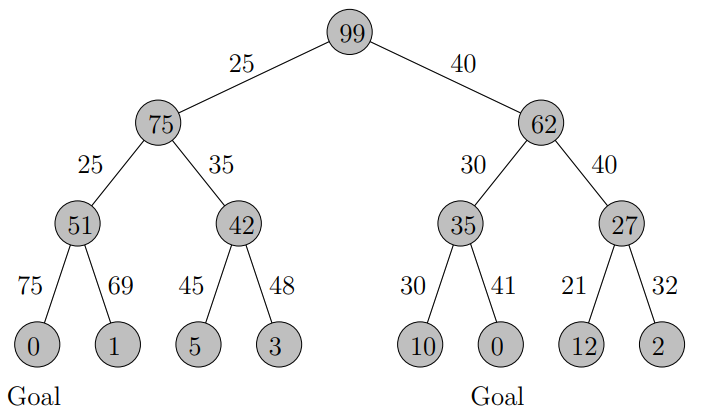
\includegraphics[width=0.45\textwidth]{searchtree}
\end{figure}

\begin{figure}[H]
\centering
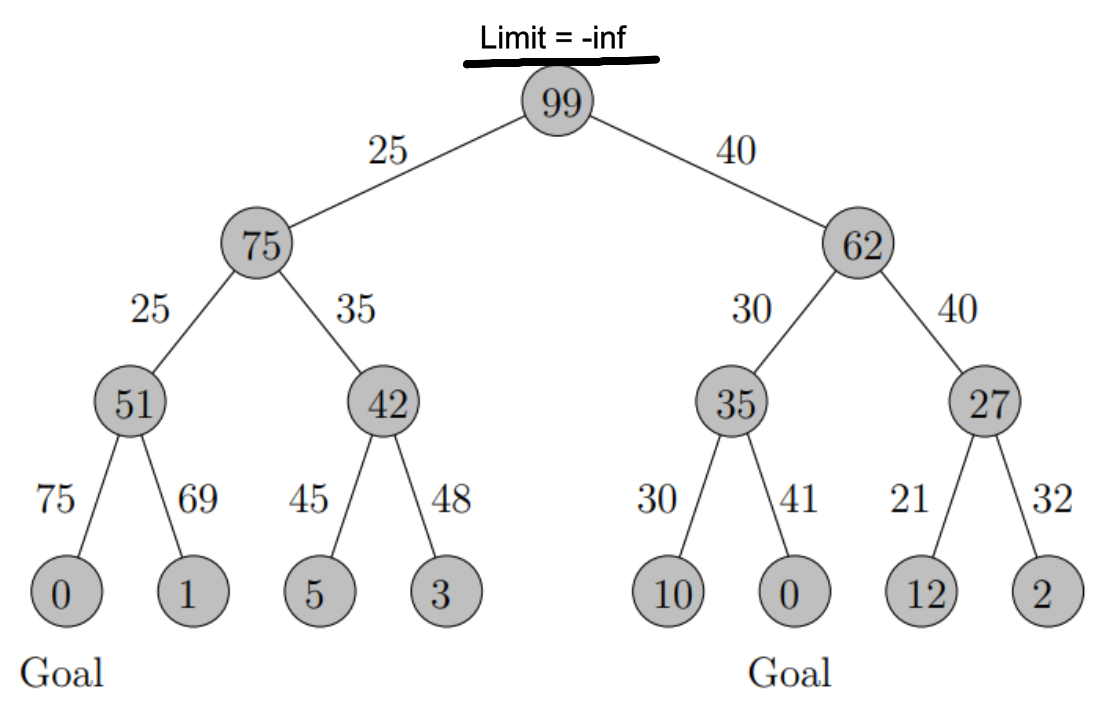
\includegraphics[width=0.45\textwidth]{searchtree1}
\end{figure}

\begin{figure}[H]
\centering
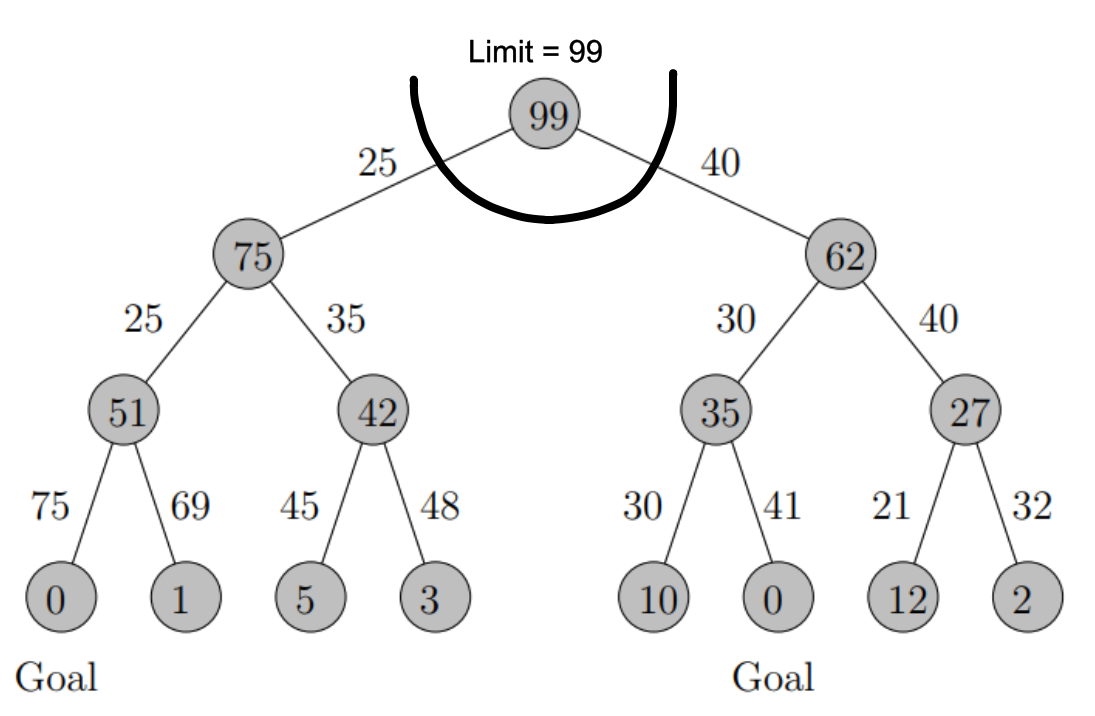
\includegraphics[width=0.45\textwidth]{searchtree2}
\end{figure}

\begin{figure}[H]
\centering
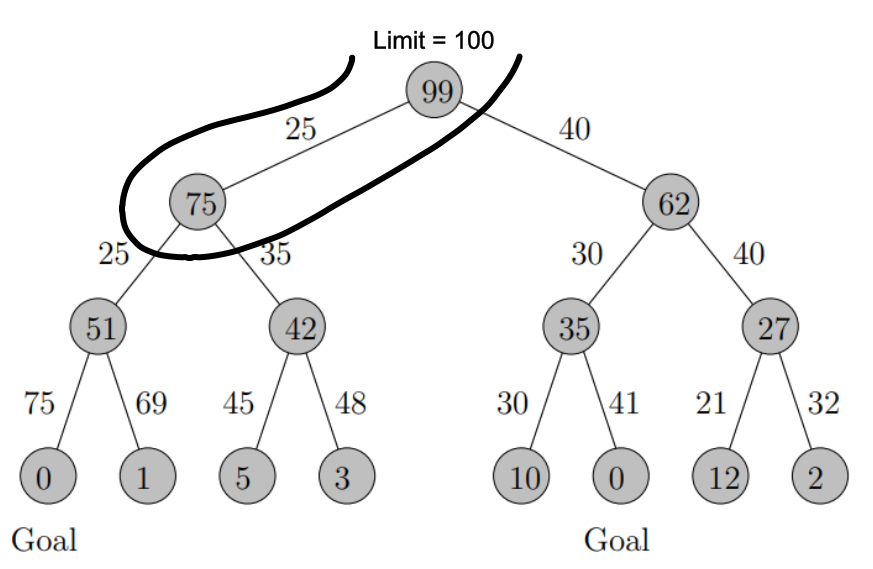
\includegraphics[width=0.45\textwidth]{searchtree3}
\end{figure}

\begin{figure}[H]
\centering
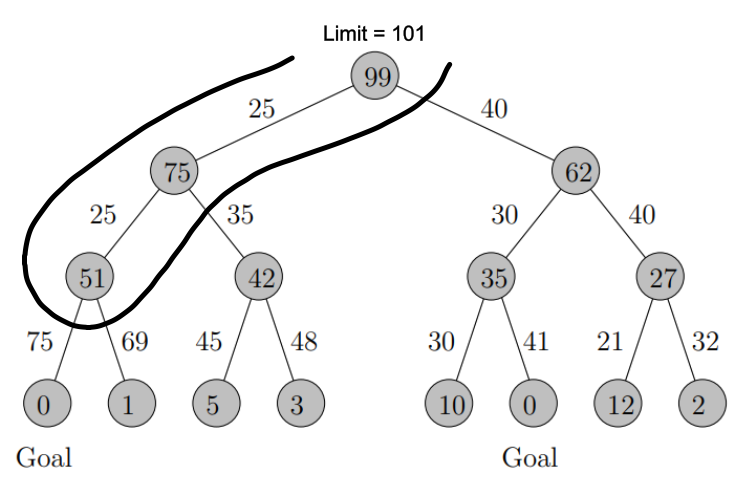
\includegraphics[width=0.45\textwidth]{searchtree4}
\end{figure}

\begin{figure}[H]
\centering
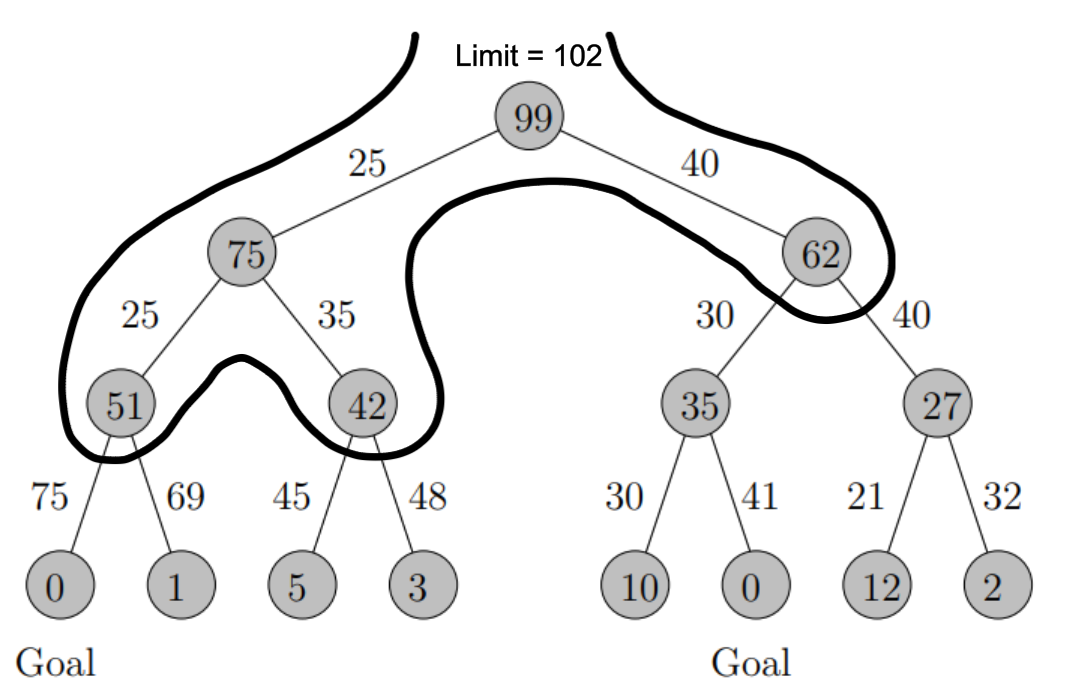
\includegraphics[width=0.45\textwidth]{searchtree5}
\end{figure}

\begin{figure}[H]
\centering
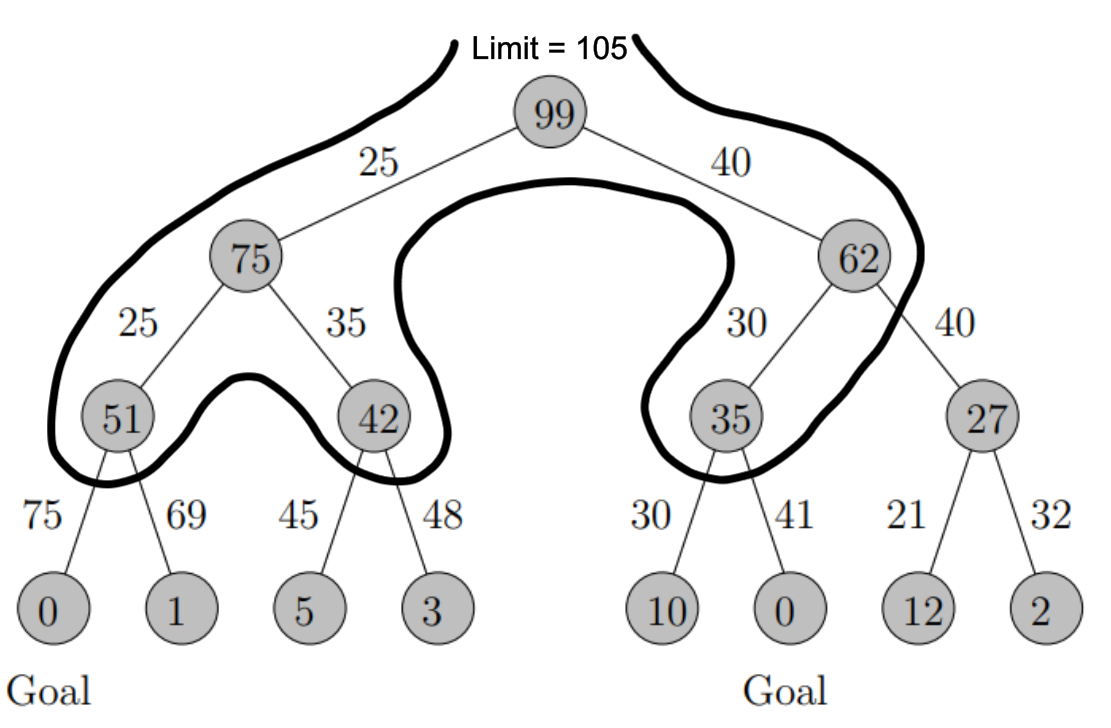
\includegraphics[width=0.45\textwidth]{searchtree6}
\end{figure}

\begin{figure}[H]
\centering
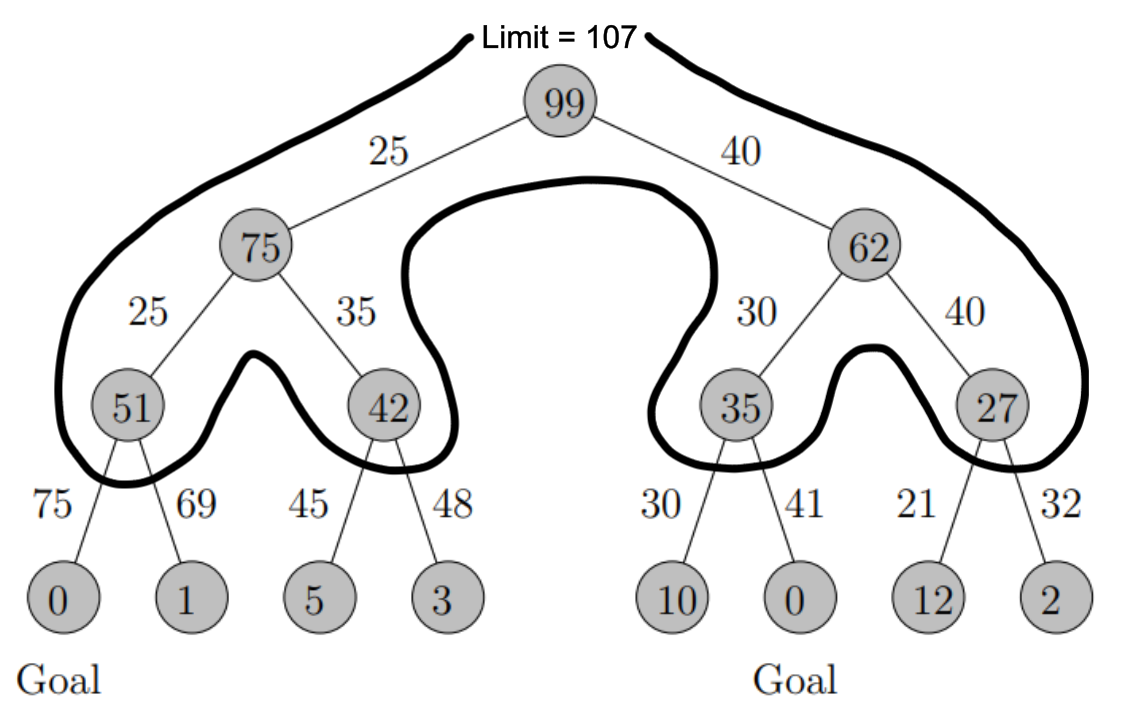
\includegraphics[width=0.45\textwidth]{searchtree7}
\end{figure}

\begin{figure}[H]
\centering
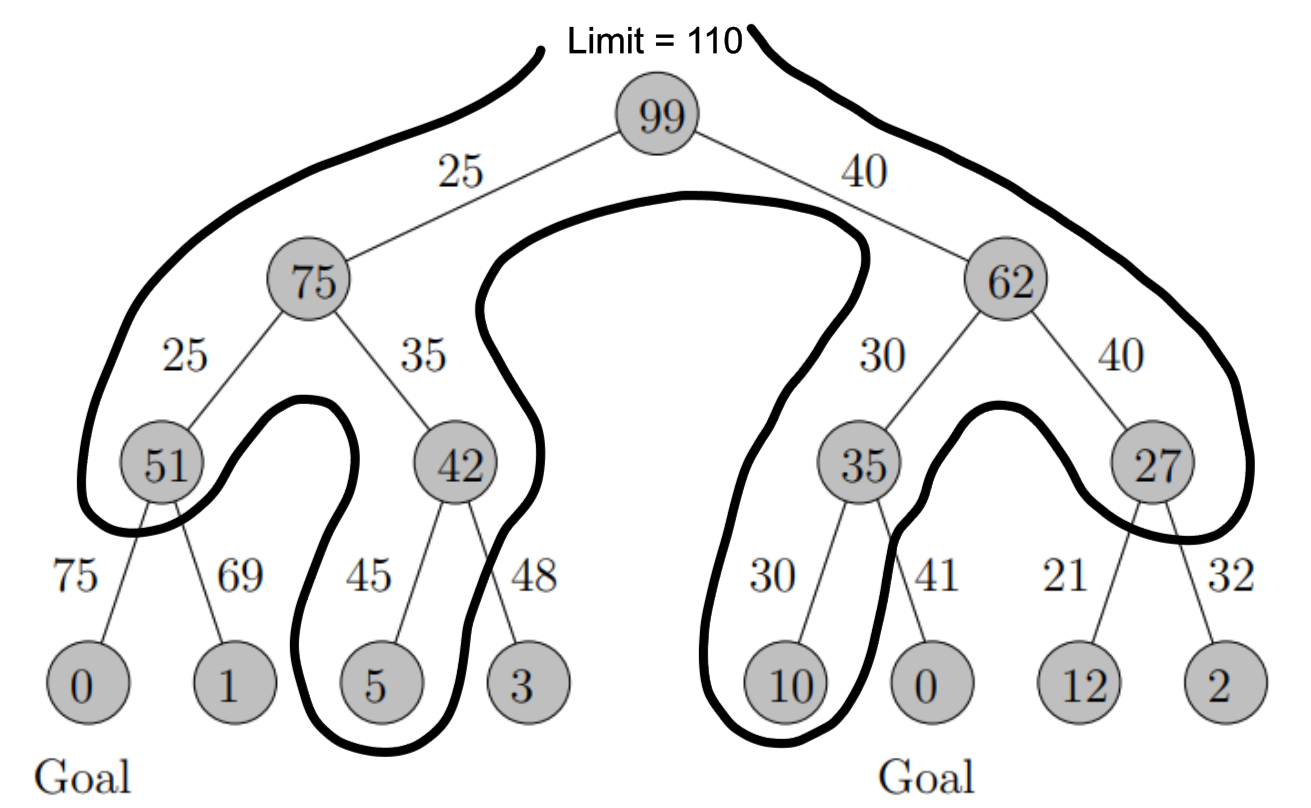
\includegraphics[width=0.45\textwidth]{searchtree8}
\end{figure}

\begin{figure}[H]
\centering
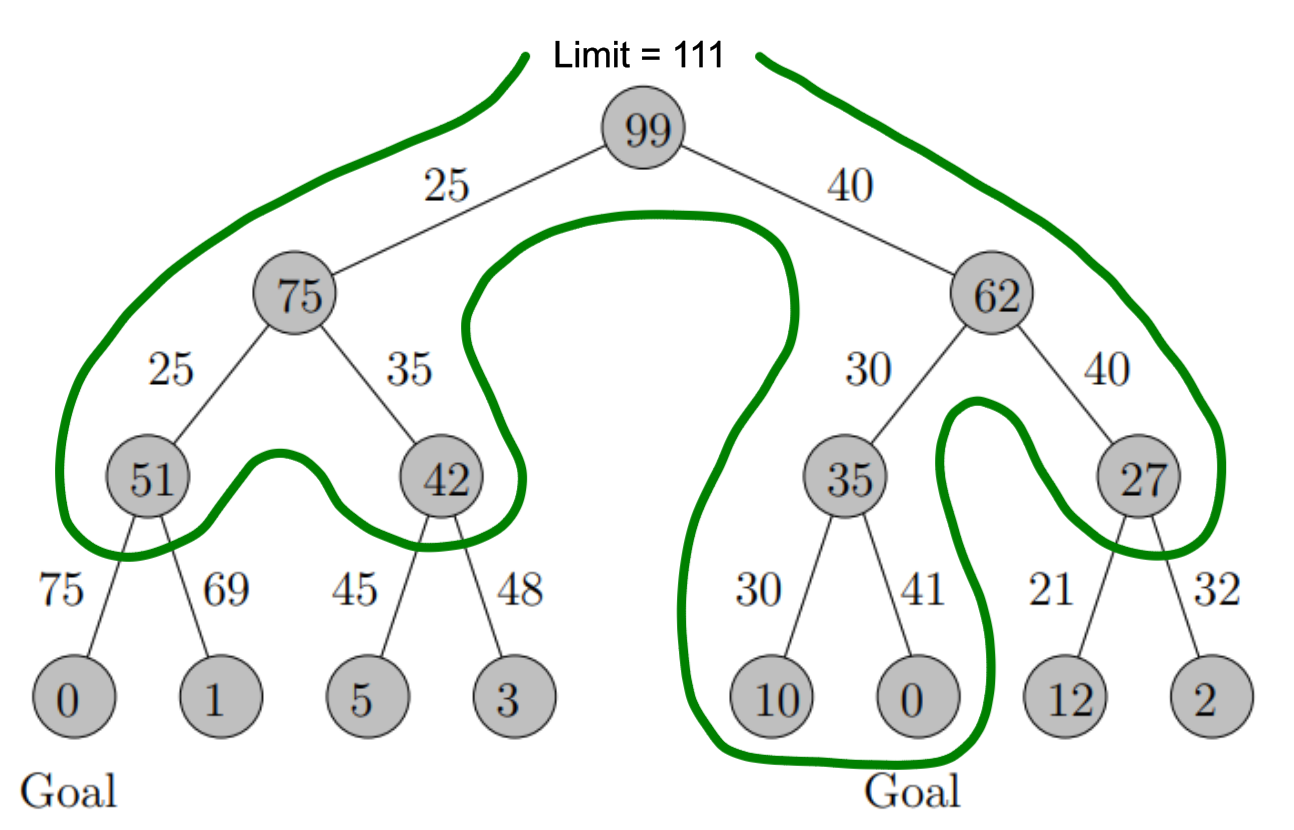
\includegraphics[width=0.45\textwidth]{searchtree9}
\end{figure}

\item Give \textit{two} reasons why the IDA$^*$ algorithm might prove
unsuitable as a solution to a search problem, in each case giving a brief
explanation of why this is the case and suggesting a potential solution.

If either of the following conditions are met then \idastar may fail to
find any solution:
\begin{itemize}

\item Edges have no minimum cost.

In this case, \idastar can keep exploring a path which tends to a value
lower than that of the optimum solution. We can solve this by constraining
all edges to have a cost $\geq \varepsilon$ for some arbitrarily small
$\varepsilon$.

\item Nodes can have an infinite number of neighbours.

In this case, once a node is expanded, the search algorithm will keep
checking all of its neighbours. In the case that none of them are goal
states, this leads to an infinite search.

In this case, the problem is not suited to a tree-search approach. There may
be some domain-specific solutions; however there is no general approach
which makes this solvable.

\end{itemize}

In the following two cases, \idastar will not be efficient:
\begin{itemize}

\item nodes have unique $f$-values

In this case, every successive call to \idastar will search \textit{one more
node}. This means the time required to find a solution is quadratic in the
number of nodes with $f$-value smaller than it. In large trees, this makes
the problem almost intractable.

This can be solved by increasing the $f$-limit by some arbitrarily small
$\varepsilon$, yielding a goal state which is guaranteed to have a cost within
$\varepsilon$ of the optimal goal state.

\item too many nodes share the same $f$-value

In this case, successive calls to \idastar will dramatically increase the
size of the tree -- rendering the search process incredibly inefficient and
similar to a complete search.

\end{itemize}

\end{enumerate}

\end{examquestion}

\begin{examquestion}{2017}{4}{1}

\texttt{EvilRobot} has two dogs called \texttt{Fido} and \texttt{Fifi}. All
three of them enjoy \texttt{pie} and \texttt{sausages} so much that they
like to steal them. At the beginning of the day the \texttt{butcher} has some
\texttt{sausages} and the \texttt{pieShop} has some \texttt{pie}. Also,
\texttt{EvilRobot} and his pets are at home, but they aim to end the day
having relieved the local businesses of their products.

\begin{enumerate}[label=(\alph*)]

\item Give a detailed definition of a \textit{Constraint Satisfaction
Problem (CSP)}. Include in your answer a definition of what it means for an
assignment to be \textit{consistent} and to be \textit{complete}, and for an
assignment to be a \textit{solution}.

A constraint satisfaction problem is the problem of assigning values $D_1,
\dots, D_n$ to a set of variables $V_1, \dots, V_n$ such that all
constraints $C_1, \dots C_m$ are met.

An assignment is consistent if it violates no constraints. An assignment is
complete if it assigns a value to every variable. An assignment is a
solution if it is both consistent and complete.

\item Consider the constraint $C$ on four variables $\{V_1, V_2, V_3, V_4\}$
each of which has the domain \texttt{\{true, false\}}, with
\[
\begin{split}
C = \{
&(\texttt{true}, \texttt{true}, \texttt{true}, \texttt{true})\\
&(\texttt{true}, \texttt{false}, \texttt{true}, \texttt{false})\\
&(\texttt{false}, \texttt{true}, \texttt{false}, \texttt{false})\\
&(\texttt{false}, \texttt{false}, \texttt{false}, \texttt{true})\\
&(\texttt{false}, \texttt{false}, \texttt{true}, \texttt{true})\}
\end{split}
\]
Explain how this constraint can be replaced by a collection of binary
constraints having an identical effect.

This constraint can be replaced by a collection of binary constraints by
introducing an auxiliary variable $A$ which takes a value from $\{1, 2, 3,
4\}$ and is $i$ if the $i^{\text{th}}$ formula is being satisfied.

\[
\begin{split}
C = \{&
(A = 0, V_1 = \texttt{true}),
(A = 0, V_2 = \texttt{true}),
(A = 0, V_3 = \texttt{true}),
(A = 0, V_4 = \texttt{true}), \\
&
(A = 1, V_1 = \texttt{true}),
(A = 1, V_2 = \texttt{false}),
(A = 1, V_3 = \texttt{true}),
(A = 1, V_4 = \texttt{false}), \\
&
(A = 2, V_1 = \texttt{false}),
(A = 2, V_2 = \texttt{true}),
(A = 2, V_3 = \texttt{false}),
(A = 2, V_4 = \texttt{false}), \\
&
(A = 3, V_1 = \texttt{false}),
(A = 3, V_2 = \texttt{false}),
(A = 3, V_3 = \texttt{false}),
(A = 3, V_4 = \texttt{true}), \\
&
(A = 4, V_1 = \texttt{false}),
(A = 4, V_2 = \texttt{false}),
(A = 4, V_3 = \texttt{true}),
(A = 4, V_4 = \texttt{true})\}
\end{split}
\]

\item Describe the state-variable representation for planning problems.
Illustrate your answer by showing how the action of \texttt{EvilRobot} (or one
of his pets) stealing something could be represented in the scenario set out
at the beginning of this question.

% TODO

\item Explain how the \textit{state} of a planning problem can be
represented in the state-variable representation.

% TODO

\item Using your example of the stealing action provided in part (c),
explain how this planning problem might be translated into a CSP. You
should include in your explanation examples of the translation for actions,
state variables, and action preconditions and action effects, but you need
not describe the translation for frame axioms.

% TODO

\end{enumerate}

\end{examquestion}

\end{document}

\iffalse

I'm a bit confused about the difference between gashnigs algorithm and
graph-based backjumping.

Does gaschnigs algorithm jump ONCE to the ``correct thing'' to jump to

Does Gaschnigs algorithm use forward checking or constraint propogation? Or
does it just ``try a value'' and if it fails then jump back to the most
recent vertex which shares an edge with the vertex on which our assignment
fails.

While graph-based backjumping does use forward checking / constraint
propagation to do a lot of small jumps to ``potentially incorrect'' things
to backjump to?

Because the parent MAY NOT BE THE FIRST THING WHICH CONFLICTED WITH THE NODE

Why is RBFS ``red code'' needed

\fi